\documentclass[11pt, a4paper, titlepage, block]{article}
\usepackage{listings}
\hyphenpenalty=10000

\begin{document}
	\begin{titlepage}
		
		\newcommand{\HRule}{\rule{\linewidth}{0.5mm}} % Defines a new command for the horizontal lines, change thickness here
		
		\center % Center everything on the page
		
		%----------------------------------------------------------------------------------------
		%        HEADING SECTIONS
		%----------------------------------------------------------------------------------------
		
		\textsc{\LARGE University of Urbino}\\[1.5cm] % Name of your university/college
		\textsc{\Large applied computer science}\\[0.5cm] % Major heading such as course name
		\textsc{\large Procedural and logic programming}\\[0.5cm] % Minor heading such as course title
		
		%----------------------------------------------------------------------------------------
		%        TITLE SECTION
		%----------------------------------------------------------------------------------------
		
		
		\HRule \\[0.4cm]
		{ \huge \bfseries Report}\\[0.2cm] % Title of your document
		\HRule \\[0.4cm]
		\textsc{\large Project for the 2014/2015 winter session}
		\\[2cm]
		%----------------------------------------------------------------------------------------
		%        AUTHOR SECTION
		%----------------------------------------------------------------------------------------
		
		\begin{minipage}{\textwidth}
			\begin{flushleft}
				\emph{Studente:}\\
				Marco \textsc{Tamagno}\\ % Your name
				matricola no: 261985
				\\[1cm]
				\emph{Studente:}\\
				Francesco \textsc{Belacca}\\ % Your name
				matricola no: 260492\\
			\end{flushleft}
		\end{minipage}\\[1cm]
		
		\begin{minipage}{\textwidth}
			\begin{flushright}
				\emph{Lecturer:} \\
				Marco \textsc{Bernardo}\\ % Supervisor`s Name
			\end{flushright}
		\end{minipage}\\[5cm]

		{\today}\\[1cm]


		%----------------------------------------------------------------------------------------
		%        DATE SECTION
		%----------------------------------------------------------------------------------------
		
	 % Date, change the \today to a set date if you want to be precise		
		%----------------------------------------------------------------------------------------
		%        LOGO SECTION
		%----------------------------------------------------------------------------------------		
		%\includegraphics{Logo}\\[1cm] % Include a department/university logo - this will require the graphicx package		
		%----------------------------------------------------------------------------------------		
		\newpage
		\tableofcontents
		\newpage
		
	\end{titlepage}
	
	\section{Specifica del Problema}
	Write an ANSI C library that manages binary relations by exporting the following functions. The first C function returns a binary relation introduced through the keyboard. The second C function has a binary relation as input parameter and prints it to the screen. The third C function has a binary relation as input parameter and establishes whether it is a partial order relation, printing to the screen which property does not hold in the case that the relation is not such. The fourth C function has a binary relation as input parameter and establishes whether it is a total order relation, printing to the screen which property does not hold in the case that the relation is not such. The fifth C function has a binary relation as input parameter and establishes whether it is an equivalence relation, printing to the screen which property does not hold in the case that the relation is not such. The sixth C function has a binary relation as input parameter and establishes whether it is a mathematical function; if it is not, then the element violating the property will be printed to the screen, otherwise a message will be printed to the screen indicating whether the function is injective, surjective, or bijective.
	[The project can be submitted also by first-year students.]\\
	\\
	Scrivere una libreria ANSI C che gestisce le relazioni binarie esportando le seguenti funzioni. La prima funzione C restituisce una relazione binaria acquisita da tastiera. La seconda funzione C ha come parametro di ingresso una relazione binaria e la stampa a video. La terza funzione C ha come parametro di ingresso una relazione binaria e stabilisce se essa `e una relazione d$'$ ordine parziale, stampando a video quale propriet`a non vale nel caso la relazione non sia tale. La quarta funzione C ha come parametro di ingresso una relazione binaria e stabilisce se essa `e una relazione d$'$ ordine totale, stampando a video quale propriet`a non vale nel caso la relazione non sia tale. La quinta funzione C ha come parametro di ingresso una relazione binaria e stabilisce se essa `e una relazione d$'$ equivalenza, stampando a video quale proprieta` non vale nel caso la relazione non sia tale. La sesta funzione C ha come parametro di ingresso una relazione binaria e stabilisce se essa `e una funzione matematica; se non lo `e, allora si stampera` a video quale elemento violi la propriet`a, altrimenti si stamper`a a video un messaggio che indica se la funzione `e iniettiva, suriettiva o biiettiva.
	[Il progetto pu`o essere consegnato anche da studenti del primo anno.]\\
	\newpage
	\section{Analisi del Problema}
	\subsection{Input}
	
	
	1. Per l$'$ acquisizione come input abbiamo una relazione binaria del tipo (a,b) che viene   acquisita da tastiera;\\
	2. Come input per le altre 5 funzioni abbiamo una relazione(precedentemente esportata dalla prima).\\
	\subsection{Output}
	
	
	1. La prima funzione(Acquisizione) restituisce una funzione binaria acquisita da tastiera;\\
	\\
	2. La seconda funzione(Stampa) non restituisce nulla, ma stampa a video la relazione che aveva in ingresso;//
	\\
	3. La terza funzione "ordine parziale" non restituisce nulla, ma stampa a video se la Relazione binaria acquisita \`e di ordine parziale o meno e stampa a video le propiet\`a della funzione, per poter mostrare a schermo quali popiet\`a non vengono rispettate;\\
	\\
	4. La quarta funzione (ordine totale) non restituisce nulla, ma stampa a video se la Relazione binaria acquisita \`e di ordine totale o meno,stampando a video quale proprieta$'$  non vale nel caso la relazione non sia tale;\\
	\\
	5. La quinta funzione(relazione equivalenza) non restituisce nulla, ma stampa a video se la relazione binaria acquisita \`e una relazione di equivalenza o meno e stampa a video le propiet\`a della funzione, per poter mostrare a schermo quali popiet\`a non vengono rispettate;\\
	\\
	6. la sesta funzione(check funzione) non restituisce nulla, ma stampa a video se la relazione binaria acquisita \`e una funzione, e in caso contrario stampa a video quale coppia non fa rispettare le propiet\`a.\\
	
	
	
	\newpage                        
	\section{Progettazione dell$'$ Algoritmo}
	\subsection{Teoria}
	Per lo sviluppo di questo programma si necessita di alcuni cenni di Teoria degli insiemi quali:\\
	\\
	Concetto di Relazione Binaria : In matematica, una relazione binaria definita su di un insieme, anche detta relazione o corrispondenza tra due oggetti, \`e un elenco di coppie ordinate di elementi appartenenti all`insieme. In modo equivalente, una relazione binaria \`e un sottoinsieme del prodotto cartesiano di un insieme con se stesso.\\
	\\
	Concetto di Relazione d$'$ Ordine Parziale: In matematica, più precisamente in teoria degli ordini, una relazione d`ordine o ordine su di un insieme \`e una relazione binaria tra elementi appartenenti all`insieme che gode delle seguenti propriet\`a:\\
	* riflessiva\\
	* antisimmetrica\\
	* transitiva.\\
	\\
	Concetto di Relazione d$'$ Ordine Totale: Una relazione d$'$ ordine si dice Totale, quando oltre a essere parziale soddisfa anche la propiet\`a di Dicotomia ( tutti gli elementi devono essere in relazione tra di loro ).\\
	\\
	Concetto di riflessivit\`a : In logica e in matematica, una relazione binaria R in un insieme X \`e detta riflessiva se ogni elemento di X \`e in tale relazione con se stesso.        \\
	\\
	Concetto di transitivit\`a: In matematica, una relazione binaria R in un insieme X \`e transitiva se e solo se per ogni a, b, c appartenenti ad X, se a \`e in relazione con b e b \`e in relazione con c, allora a \`e in relazione con c. \\
	\\
	Concetto di simmetricit\`a: In matematica, una relazione binaria R in un insieme X \`e simmetrica se e solo se, presi due elementi qualsiasi a e b, vale che se a \`e in relazione con b allora anche b \`e in relazione con a.\\
	\\
	Concetto di funzione: In matematica, una funzione, anche detta applicazione, mappa o trasformazione, \`e definita dai seguenti oggetti:\\
	* Un insieme  X  detto dominio della funzione.
	* Un insieme  Y  detto codominio della funzione.
	* Una relazione  f : X -> Y  che ad ogni elemento dell`insieme  X  associa uno ed un solo elemento dell`insieme  Y ; l`elemento assegnato a  x appartenente ad X  tramite  f  viene abitualmente indicato con  f(x) .\\
	\newpage
	
	Concetto di Iniettivit\`a: Una funzione si dice iniettiva quando a ogni elemento del dominio \`e assegnato uno e uno solo elemento del codominio.\\
	\\
	Concetto di Suriettivit\`a: Una funzione si dice suriettiva quando ogni elemento del codominio viene raggiunto da un elemento del dominio.\\
	\\
	\newpage        
	\subsection{Funzioni per l`acquisizione:}
	
	acquisizione() : per acquisire la relazione.\\
	\\
	
	\subsection{Funzioni per la verifica delle propriet\`a:}

	check\textunderscore iniettivita() : per controllare se l$'$ iniettivit\`a \`e rispettata o meno (0 non c$'$ \`e, 1 c$'$ \`e).\\
	\\
	check\textunderscore transitivita() : per controllare se la transitivit\`a 
	viene rispettata o meno (0 non c$'$ \`e, 1 c$'$ \`e).\\
	\\
	check\textunderscore simmetria() : per controllare se la simmetria viene rispettata o meno (0 non c$'$ \`e, 1 c$'$ \`e).\\
	\\
	check\textunderscore riflessivita() : per controllare se la riflessivit\`a viene rispettata o meno (0 non c$'$ \`e, 1 c$'$ \`e).\\
	\\
	check\textunderscore dicotomia() : per verificare se la dicotomia viene rispettata o meno (0 non c$'$ \`e, 1 c$'$ \`e).\\
	\\
	check\textunderscore suriettivita(): verifica se la funzione gode della propriet\`a di suriettivit\`a, in questo caso sar\`a sempre settata a 1 in quanto tutti gli elementi del codominio (presi come gli elementi dei vari secondi termini digitati durante l$'$ acquisizione) avranno sempre un elemento del dominio associato(dato che non si pu\`o acquisire il secondo termine se non se ne acquisice prima il relativo primo, o arrivare alla funzione check\textunderscore suriettivita() avendo acquisito solo il primo).\\
	\\
	\newpage
	\subsection{Funzioni principali:}
	ordine\textunderscore parziale() : richiama le funzioni delle propriet\`a e controlla se c$'$ \`e un ‘ordine parziale(stampa a video se c$'$ \`e o meno un ordine parziale, e nel caso non c$'$ \`e stampa quali propriet\`a non vengono rispettate).\\
	\\
	ordine\textunderscore totale(): richiama la funzione ordine\textunderscore parziale e check\textunderscore dicotomia e controlla se c$'$ \`e un ordine totale(stampa a video se esiste o meno un ordine totale, e nel caso non c$'$ \`e stampa quali propiet\`a non vengono rispettate).\\
	\\
	relazione\textunderscore equivalenza() : richiama le funzioni delle propriet\`a e controlla se c$'$ \`e una relazione d$'$ equivalenza(stampa a video se c$'$ \`e o meno una relazione d$'$ equivalenza, e nel caso non c$'$ \`e stampa quali propriet\`a non vengono rispettate).\\
	\\
	check\textunderscore funzione():verifica se la relazione \`e una funzione(stampa  a video se c$'$ \`e o non c$'$ \`e una funzione e nel caso non ci sia dice quale coppia non soddisfa le propriet\`a).\\
	\\
	\newpage        
	\subsection{Input}
	
	
	Per l$'$ input abbiamo necessit\`a di usare una struttura dati dinamica, nella quale andiamo a salvare la Relazione Binaria dataci dall$'$ utente, il numero delle coppie e il tipo di input ( numerico o per stringhe).\\
	\\
	L input dovr\`a essere dotato di diversi controlli, se l$'$ utente sceglie di inserire un input di tipo numerico allora non potra digitare stringhe e/o caratteri speciali etc.\\
	\\
	La scelta di due tipi di input differente dovr\`a essere data per dare la possibilit\`a all$'$ utente nel caso scelga di fare un$'$ input di tipo numerico di poter effettuare operazioni non legate alle funzioni della libreria, (esempio : l$'$ utente vuole decidere di moltiplicare l$'$ input per due, e vedere se mantiene le propiet\`a, con un$'$ input di tipo numerico l$'$ utente può farlo e ciò avrebbe un senso, con un$'$ input di tipo stringa meno).\\
	\\
	La scelta dell$'$ input di tipo stringa dovr\`a essere data per aver maggior completezza, una relazione binaria non deve essere forzatamente numerica ma può essere anche tra cose, oggetti, animali, colori e qualsiasi altra cosa possa venire in mente.\\
	\\
	Alle varie funzioni verr\`a data come input la struttura dati salvata in precedenza dalla funzione Acquisizione, per poterne verificare le varie propiet\`a.\\
	
	
	
	
	\newpage        
	\subsection{Output - Acquisizione}
	Durante l$'$ acquisizione avremo diversi output video (printf) che guideranno l$'$ utente nell$'$ inserimento dei dati, e che segnaleranno eventuali errori commessi.
	Finita l$'$ acquisizione dovremo restituire l$'$ indirizzo della struttura, che all$'$ interno quindi conterra$'$  i dati inseriti dall$'$ utente. Abbiamo scelto di fare ciò perch\`e non essendo permesso l$'$ utilizzo di variabili globali, il modo più semplice di passare i dati inseriti da una funzione all$'$ altra e$'$  quello di creare una struttura dinamica.
	Una volta restituito l$'$ indirizzo della struttura, a seconda della funzione lanciata nel file Test.c si lanceranno le altre 5 funzioni, dato che queste prendono tutte in pasto l$'$ output della prima (cio\`e l$'$ indirizzo della struttura della relazione binaria) e la utilizzano per verificarne varie proprieta$'$ .\\
	\\
	\subsection{Output - stampa}
	La funzione “stampa” avra$'$  come output la stampa a video della struttura acquisita, con qualche aggiunta grafica(le parentesi e le virgole) per rendere il tutto più facilmente interpretabile e leggibile.\\
	\\
	\subsection{Output - ordine\textunderscore parziale}
	La funzione “ordine\textunderscore parziale” avra$'$  come output la stampa a video del risultato della verifica delle proprieta$'$  di riflessivita$'$  antisimmetria e transitivita$'$ . Nel caso in cui siano tutte verificate si stampera$'$  che la relazione e$'$  una relazione di ordine parziale, mentre nel caso in cui non siano verificate si stampera$'$  che non lo e$'$  e il perche$'$  (cioe$'$  quale proprieta$'$  non e$'$  o non sono verificate).\\
	\\
	\subsection{Output - ordine\textunderscore totale}
	La funzione “ordine\textunderscore totale” avra$'$  come output la stampa a video del risultato della verifica delle proprieta$'$  necessarie ad avere una relazione d$'$ ordine parziale, e verifichera$'$  poi se anche la dicotomia \`e valida per la relazione o meno. Nel caso in cui tutto sia positivo, allora si stampera$'$  che la relazione e$'$  di ordine totale, mentre se non lo e$'$  si stampera$'$  cosa fa in modo che non lo sia.\\
	\\
	\subsection{Output - relazione\textunderscore equivalenza}
	La funzione “relazione\textunderscore equivalenza” avra$'$  come output la stampa a video del risultato della verifica delle proprieta$'$  di riflessivita$'$  simmetria e transitivita$'$  e nel caso in cui siano tutte positive si stampera$'$  che la relazione e$'$  una relazione di equivalenza, mentre nel caso in cui qualcosa non sia verificato si stampera$'$  cio$'$  che impedisce alla relazione di essere una relazione d$'$ equivalenza.\\
	\\
	\subsection{Output - check\textunderscore funzione}
	La funzione ”check\textunderscore funzione” avra$'$  come output la stampa a video della verifica della proprieta$'$  che rende la relazione binaria una funzione, e in caso lo sia anche se questa e$'$  suriettiva(che poi spiegheremo essere sempre verificata) e iniettiva, e in caso sia entrambe si stampera$'$  che la relazione binaria oltre ad essere una funzione e$'$  una funzione biiettiva.\\
	\\
	\newpage
	\section{Implementazione dell$'$ algoritmo}
	\subsection{Libreria}
	\lstset{numbers=left, tabsize=2,breaklines=true, language=C}
	\lstinputlisting{Progetto.h} 
	\newpage
	\subsection{Test}
	\lstset{numbers=left, tabsize=2,breaklines=true, language=C}
	\lstinputlisting{Test.c}
	\newpage
	\subsection{Makefile}
	Test.exe: Test.c Makefile\\
	gcc -ansi -Wall -O Test.c -o Test.exe\\
	pulisci:\\
	rm -f Test.o\\
	pulisci\textunderscore tutto:\\
	rm -f Test.exe Test.o\\
	
	
	
	
	
	
	
	\newpage
	\section{Testing the program}
	Test 1:\\
	Test di Relazione d$'$ ordine Totale.\\
	\\
	Inputs: (a,a)(a,b)(b,b)\\
	\\
	Outputs: checkriflessivit\`a : 1,checksimmetria : 0, checktransitivit\`a : 1
	checkdicotomia : 1, la relazione \`e una relazione d$'$ ordine totale in quanto \`e rispetta anche la propiet\`a di Dicotomia.\\
	\\
	\\
	Test 2: \\
	Test di Relazione d$'$ ordine Parziale.\\
	\\
	Inputs:(a,a)(b,b)(a,b)(c,c)\\
	\\
	Outputs:checkriflessivit\`a : 1,checksimmetria : 0, checktransitivit\`a : 1
	la relazione \`e una relazione d$'$ ordine parziale in quanto rispetta le propriet\`a.\\
	\\
	\\
	Test 3: \\
	Test di Relazione d$'$ ordine non Parziale.\\
	\\
	Inputs:(a,a)(b,b)(c,c)(d,d)(e,e)(a,b)(b,c)\\
	\\
	Outputs:checkriflessivit\`a : 1,checksimmetria : 0, checktransitivit\`a : 0
	la relazione non \`e una relazione d$'$ ordine parziale in quanto non rispetta le propriet\`a.\\
	\\
	\\
	Test 4:\\
	Test di Relazione d$'$ equivalenza.\\
	\\
	Inputs:(a,a)(a,b)(b,a)(b,b)\\
	\\
	Outputs:checkriflessivit\`a : 1,checksimmetria : 1, checktransitivit\`a : 1
	checkdicotomia : 0, la relazione \`e una relazione d$'$ equivalenza in quanto rispetta le propriet\`a.\\
	\\
	\\
	Test 5:\\
	Test di Relazione non d$'$ equivalenza.\\
	\\
	Inputs:(a,a)(a,b)(b,c)\\
	Outputs:checkriflessivit\`a : 0,checksimmetria : 0, checktransitivit\`a : 0
	la relazione non \`e una relazione d$'$ ordine d$'$ equivalenza in quanto non rispetta le propriet\`a.\\
	\\
	\\
	Test 6:\\\
	Test di Funzione.\\
	\\
	Inputs:(a,a)
	Outputs:La relazione binaria e$'$  una funzione.\\
	La relazione binaria e$'$  iniettiva.\\
	La relazione binaria e$'$  biiettiva.\\
	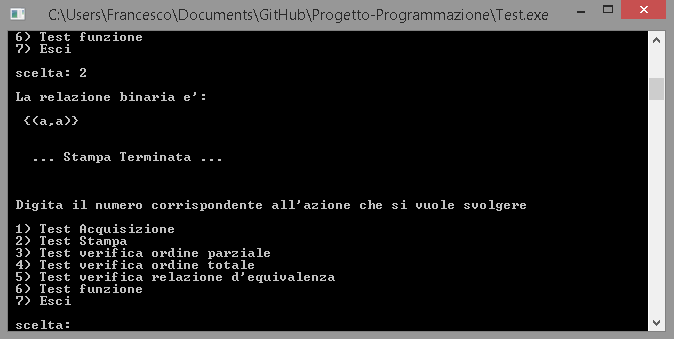
\includegraphics[width=4in,height=4in,viewport=0 0 300 300]{Test6Input.png}
	\includegraphics[width=4in,height=4in,viewport=0 0 300 300]{Tes6Output.png}
	\\
	\\
	Test 7:\\
	Test per verificare il controllo degli inputs.\\
	\\
	Inputs:(casa rossa,casa blu)(casa blu,casa blu)(casa rossa,casa rossa)\\
	\\
	Outputs:check\textunderscore riflessivit\`a : 1,check\textunderscore simmetria : 1, check\textunderscore transitivit\`a : 1 dicotomia :1
	la relazione \`e una relazione d$'$ ordine totale in quanto rispetta le propriet\`a.\\
	le funzioni funzionano anche con input contenti degli spazi.\\
	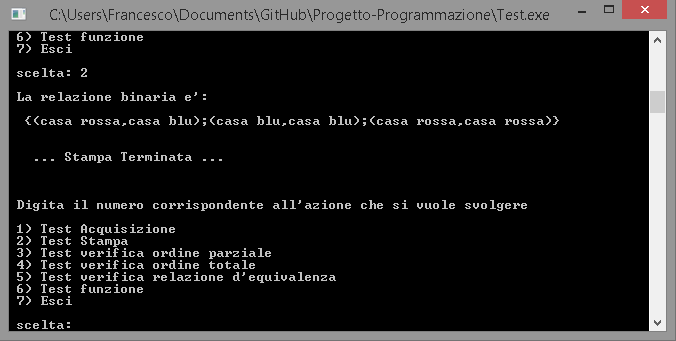
\includegraphics[width=4in,height=4in,viewport=0 0 300 300]{Test7Input.png}
	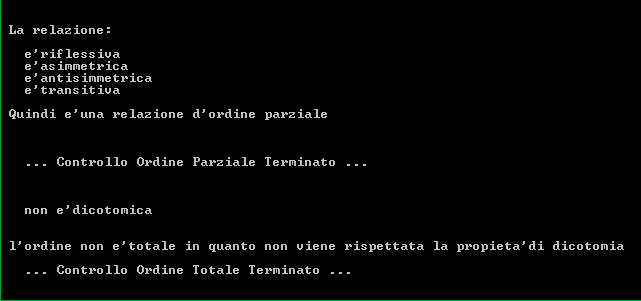
\includegraphics[width=4in,height=4in,viewport=0 0 300 300]{Test7Output.png}
	\\
	\\
	Test 8:\\
	Test per inserire stringhe in una relazione numerica.\\
	\\
	Inputs:(1,a)\\
	\\
	Outputs: c$'$ \`e un errore reinserisci il valore.\\
	\\
	stampa errore in quanto si era selezionato di voler immettere un input di tipo numerico.\\
	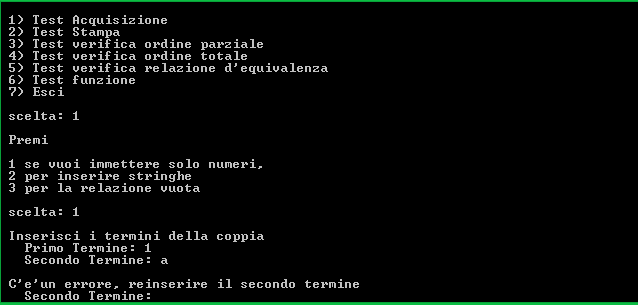
\includegraphics[width=4in,height=4in,viewport=0 0 300 300]{Test8Input.png}
	\\
	\\
	\newpage
	Test 9:\\
	Test per vedere se una relazione binaria qualunque e' una funzione.\\
	Inputs:(1,2)(1,1)\\
	\\
	Outputs: La relazione binaria non \`e una funzione\\
	Nel 2 elemento c$'$ \`e un errore che impedisce alla relazione binaria di essere una funzione;
	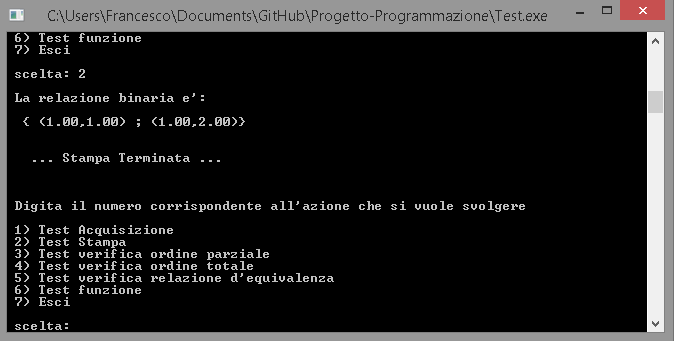
\includegraphics[width=4in,height=4in,viewport=0 0 300
	300]{Test9Input.png}
	\includegraphics[width=4in,height=4in,viewport=0 0 300
	300]{Tes9Output.png}
	\\
	\\
	Test 10:\\
	Inputs:(1,1)(2,1)\\
	\\
	Outputs: La relazione binaria e$'$  una funzione\\
	Nel 2 elemento c$'$ \`e un errore che impedisce alla funzione di essere iniettiva\\
	La funzione non e$'$  iniettiva\\
	La funzione non e$'$  biiettiva\\
	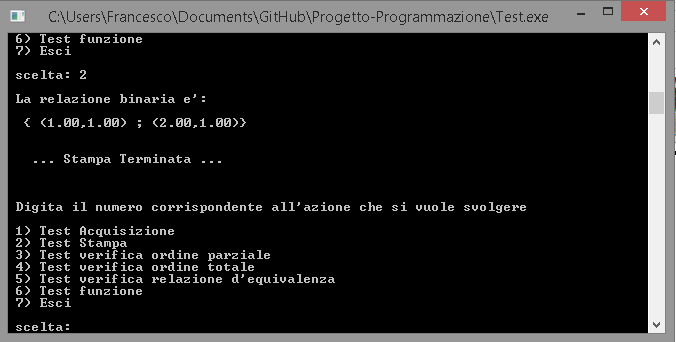
\includegraphics[width=4in,height=4in,viewport=0 0 300 300]{Test10Input.png}
	\includegraphics[width=4in,height=4in,viewport=0 0 300 300]{Tes10Output.png}
	\newpage
	\section{Verifying the program}
	
	
	
	
	
	
\end{document}

